\documentclass{article}
\usepackage[utf8]{inputenc}
\usepackage{amsmath}
\usepackage{mathtools}
\usepackage{bm}
\usepackage{graphicx}
\title{COL352: Assignment 2}
\author{Sachin 2019CS10722 }
\date{February, 2022}

\begin{document}

\maketitle


\section{Question 1}
The given language is not regular and we will prove this using the pumping lemma. \\
Given $L_1 = \{bin(p): p is a prime number\}$\\
\textbf{Proof:}\\lets assume language of binary representation of all prime numbers is regular.\\
Lets take a prime no $p \in L_1$ that ends with b 0's and a 1.since prime numbers are not divisible by 2 it ends with 1.
so our $P = x000..btimes1=xy1$ where $|x| = a,y=0 ,|y|=b$ where $b>=1.$\\
Then using pumping lemma we will have a prime q such that q=$x{y^i}1$ for any $i>=0$ .\\
Our $p=xy1$,q=$x{y^i}1$ after expanding to decimal system will be $p=+1$ and 
$q=1+{2^{ib+1}}x$ implies
$$q = p - {2^{b+1}}x + {2^{ib+1}}x $$
$$q = p +2^{b+1}x({2^{ib-1}-1})$$
Now lets take a $k \in I$ such that $({2^{ib-1}-1)}= kp$ implies
$$2^{ib-1}=kp+1$$
$$ib-1=log(kp+1)$$
$$ib=log(kp+1)+1$$
we need to choose k,p such that kp+1 is a power of 2 such that ib will be an integer.For example k=3,P=(101) in base 2=5
gives kp+1=16 we can get i=5 and b=1
So our q will be $$q=p+2^{b+1}x(kp)$$
$$q=p(1+2^{b+1}xk)$$
Implies q has factors other that 1,So q is not a prime number which contradicts pumping lemma.So given language is not regular.



\pagebreak


\section{Question 2}
\textbf{The n-th Fibonacci number is defined as \boldsymbol{$F_1 = 1, F_2 = 1$}, and for all \boldsymbol{$n \geq 3$}, \boldsymbol{$F_n = F_{n-1} + F_{n-2}$} .Consider the language over \boldsymbol{$\Sigma = \{a\}$ $L_2 = \{a^m | m = F_n \}$} Is \boldsymbol{$L_2$} regular? Justify your answer.}\\
\newline
The given language is not regular and we will prove this using the pumping lemma. \\
\textbf{To Prove:} $L_2$ is not regular.\\
\textbf{Proof:} We will use the contrapositive of the pumming lemma here. So let k be the pumping length s.t. $k\geq 1$. Now we pick a fibonacci number $F_n\geq k$ and also $F_{n+1}-F_{n}>k$. Such a fibonacci number exists clearly because second condition basically comes to $F_{n-1}>k$. So we have to find a fibonacci number which is greater than k and the fibonacci just number before it is also grater than k. That is clearly possible since fibonacci is a fast growing series.\\
Now,
\[ k\geq 1 , a^{F_n}\in L_2 \ and \ |a^{F_n}|\geq k\] 
Every break up of $a^{F_n}$ can be written as xyz :
\[x=a^r,y=a^s,z=a^t\ where \ r+s+t=F_n\] 
\[ Also, \ |xy|\leq k \ and \ y\neq \epsilon \implies  s\neq0 \ and \ s\leq k\ \ \ \ \ \ \ \  -(i)\]
Now consider i=2 . Clearly  $i\geq0$.
We can pump up y for i=2 to get:
\[xy^2z = a^{r+2*s+t}\] 
\[=> a^{F_n+s}\] 
\[We \ know \ F_n<F_n+s\leq F_n+k<F_{n+1} \ \ \ \ \ - From\ (i)\]
So we have shown that $F_n+s$ is not a fibonacci number so $xy^2z\notin L_2$ . Hence by the contrapositive of the pumping lemma $L_2$ is not a regular language. Hence Proved.

\pagebreak



\section{Question 3}
\textbf{If A is any language, let $A_{\frac{1}{2}-}$ denote the set of all first halves of strings in A so that \[ A_{\frac{1}{2}-} = \text{\{x \boldsymbol{$|$} for some \boldsymbol{$y,|x|=|y|$} and xy} \in A\} \] 
        Show that if A is regular, then so is \boldsymbol{$A_{\frac{1}{2}-}$}.\\}

To, show that $A_{\frac{1}{2}-}$ is regular, it is sufficient to show that there exist a 2DFA that accepts $A_{\frac{1}{2}-}$ (as it was proved in class that language accepted by 2DFA is regular).\\
Now, before constructing the 2DFA, consider the following psuedo code:- \\

Let DFA D accepts A, and $x \in \Sigma^*$
Start from start state of D\\
Run the string x on D\\
Suppos final state is $q_i$\\
From, $q_i$ at each step traverse to all states having 1-step transition from $q_i$\\
Iteratively, make similar transitions from all states at step i\\
Perform $|x|$ such steps\\
If out of all states in last step if any of them is in final state then x is accepted else x is rejected.\\

So, basically from state $q_i$ we are traversing all states that are $|x|$ transitions away (hence got all possible final states that we can get after running $xy$ such that $|x| = |y|$).\\
Since $\hat{\delta}(q_0,xy) = \hat{\delta}(\hat{\delta}(q_0,x),y)$\\

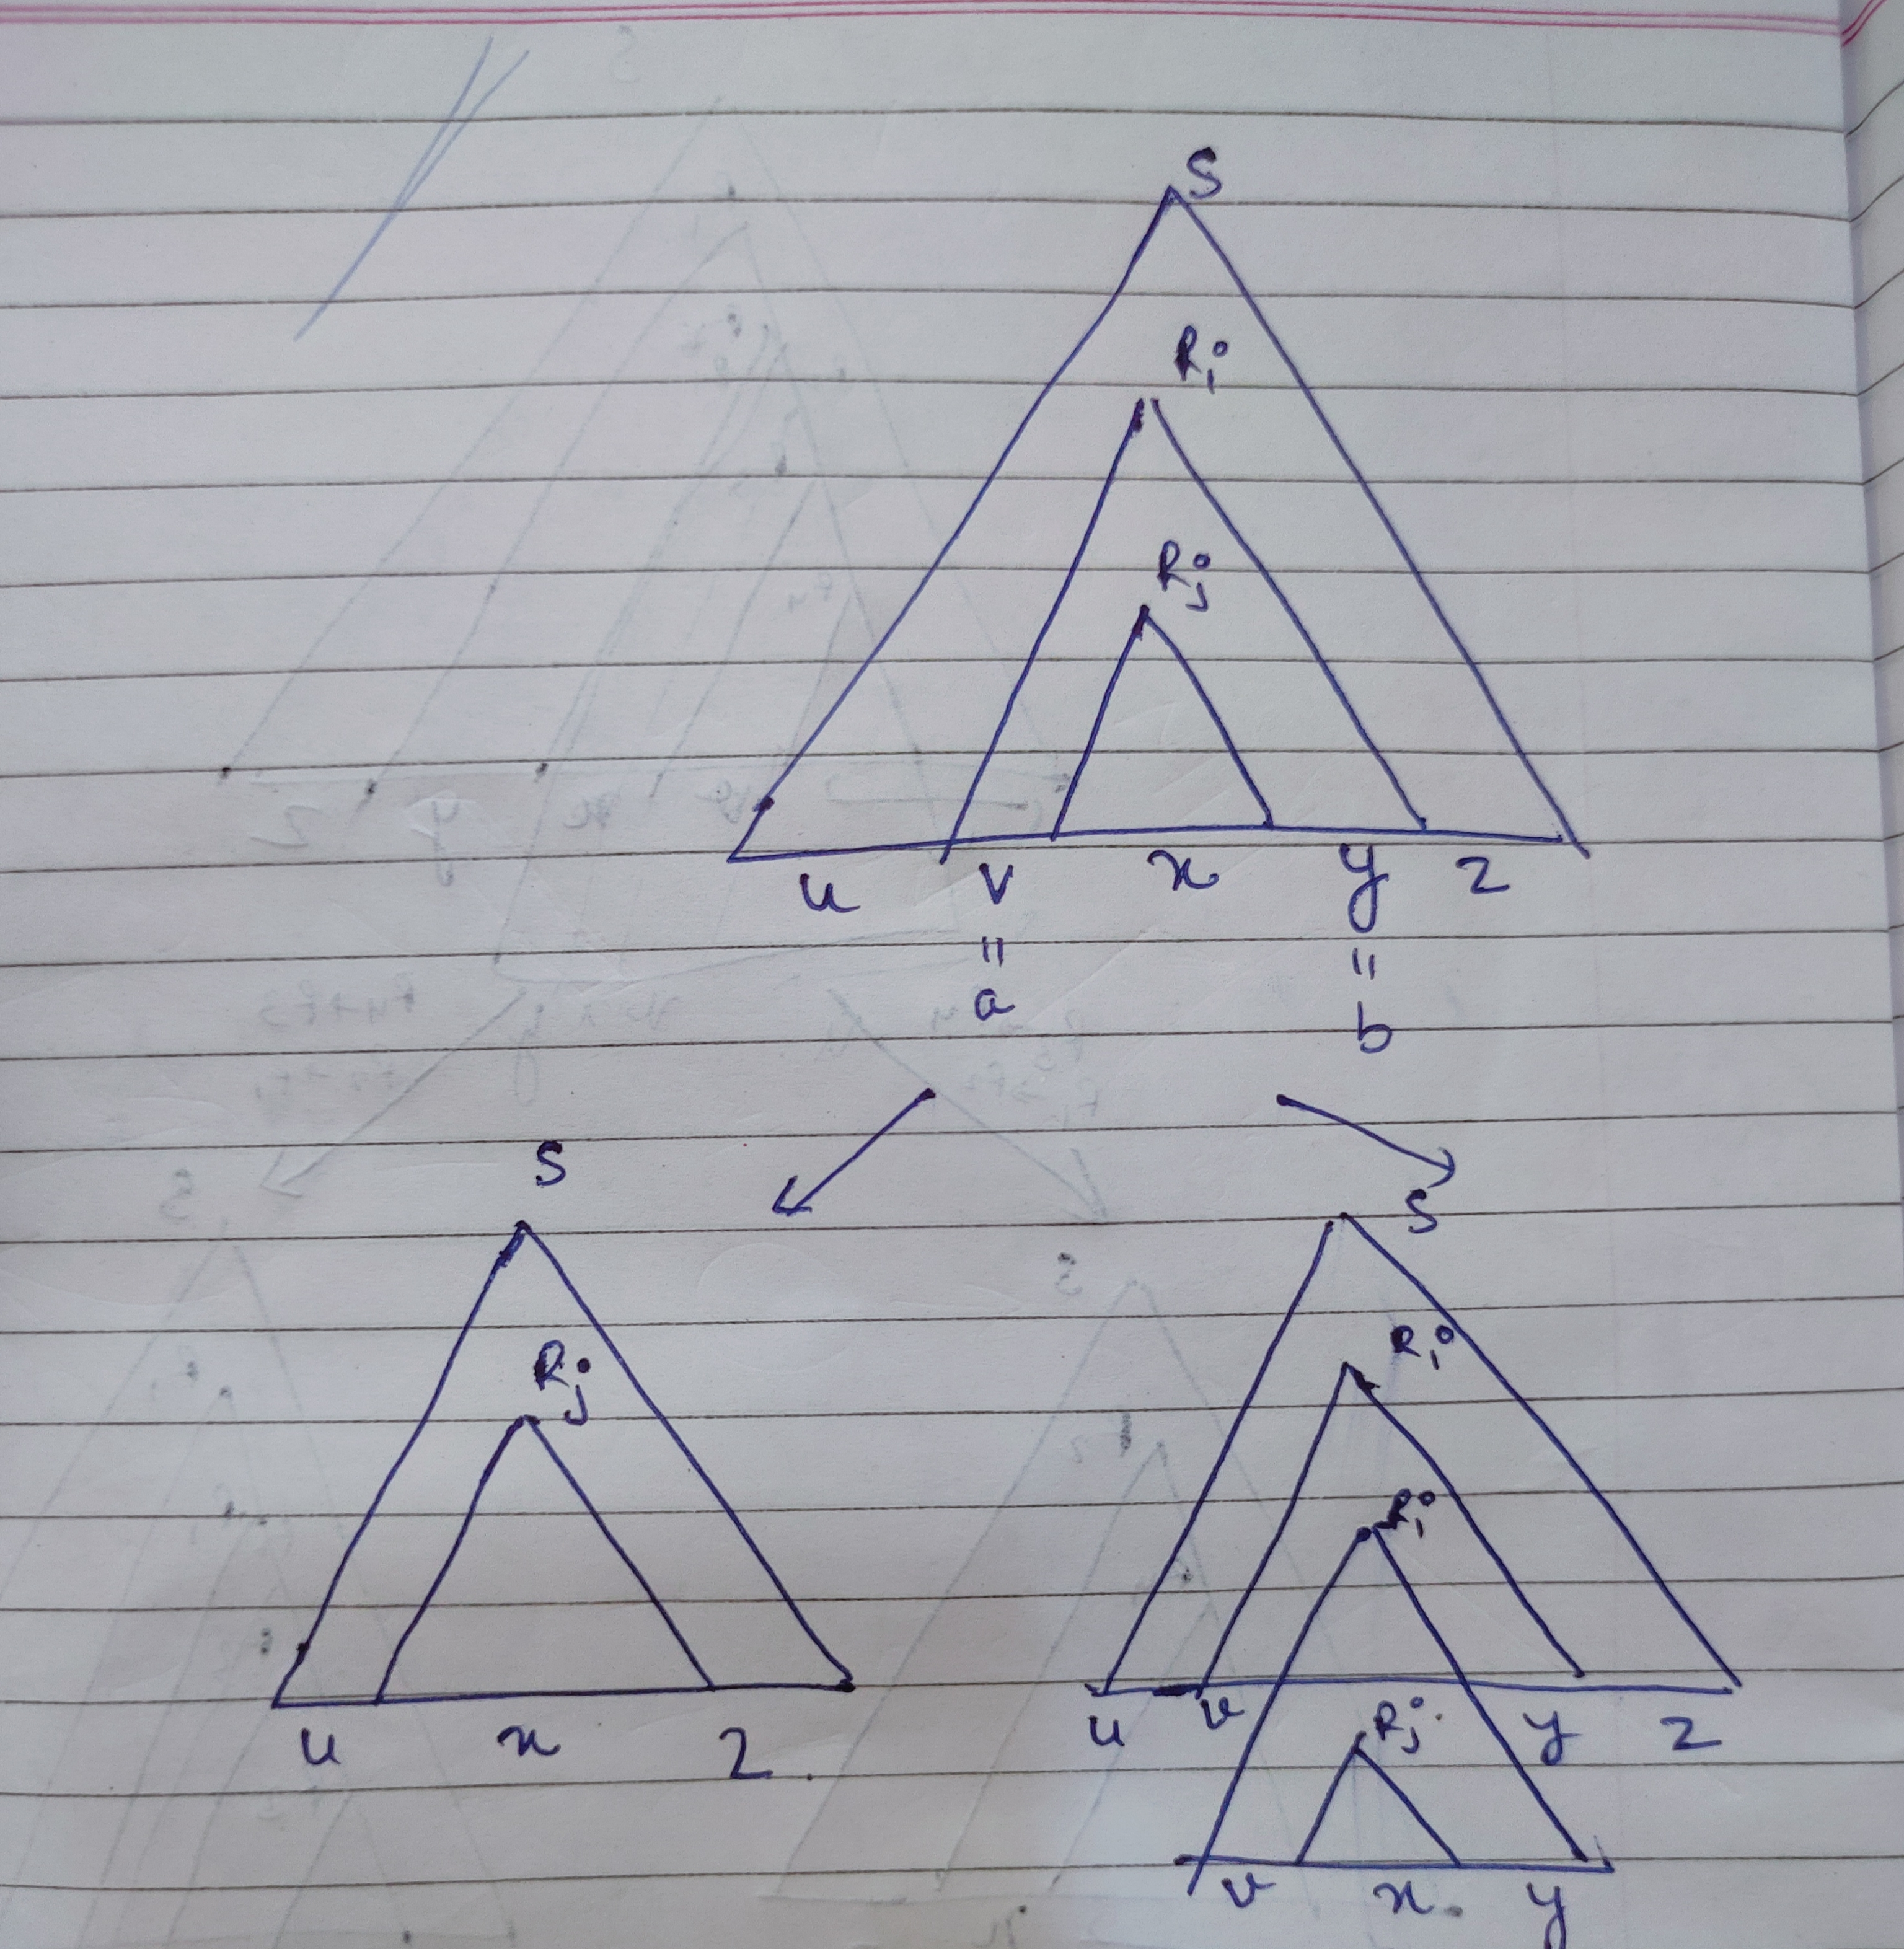
\includegraphics[width=13cm]{3.jpg}\\

Now, lets folmally define the 2DFA D' that runs above psuedo code:- 
We will require 2 DFA's D1 and D2 to construct D'.\\
Let D1 = D = $\{Q,\Sigma,\delta,q_0,F\}$\\
First run of x would be on D with transition function $\delta$ and moving right.\\
Second run would be on D2 = $\{2^Q,\Sigma,\delta_1,q_0,F'\}$ with transition function $\delta'$ and moving left.\\

So, D' = $\{Q',\Sigma \bigcup \{ \#,\$ \},\delta',q_0,q_a,q_r\}$\\ is defined as:- 
$Q' = Q \bigcup 2^Q \bigcup q_a \bigcup q_r$\\
$\delta'(q'_i,a) $ defined as:
\begin{enumerate}
    \item $q'_i \in Q$ (first run)\\
    $\delta'(q_0,\#) = (q_0,R)$\\
    $\delta'(q_i,c) = (\delta(q_i,c),R)$ if $c \in \Sigma$\\
    $\delta'(q_i,\$) = (\{q_r\},L)$\\

    \item $q'_i \in 2^Q$ (second run)\\
    $\delta'(q'_i,c) = ( \bigcup\limits_{q_k \in q'_i} \{ \bigcup\limits_{a \in \Sigma} \delta(q_i,a) \},L)$ if $c \in \Sigma$\\
    $\delta'(q'_i,\#) = (q_a,L)$ if $q'_i \bigcap F \neq \phi$\\
    $\delta'(q'_i,\#) = (q_r,L)$ if $q'_i \bigcap F = \phi$\\
\end{enumerate} 

\textbf{Claim: } Above 2DFA accepts $A_{\frac{1}{2}-}$\\
\textbf{Proof:}     
    Consider string $x \in \Sigma^*$\\
    if, $x \in A_{\frac{1}{2}-}$\\
    $<=> \exists y$ such that $ xy \in A, |x| = |y| = $ n(say)\\
    Consider the run of $xy$ on D.\\
    Let, $\hat{\delta}(q_0,x) = q_i $
    $\hat{\delta}(q_i,y) = q_j$\\
    $<=> q_j \in F$\\
    Now, consider the run of x on D' \\
    $(q_0,0) \xrightarrow{x} (q_i,n) $\\
    $(q_i,n) \xrightarrow{y} (q'_i,2n) $\\
    $q'_i$ is the set of all possible final states rechable from $q_i$ after n transition\\
    Clearly $q_j$ is in $q'_i$ (as $|y| = n$)\\
    $=> q_j \in F <=> q'_i \bigcup F \neq \phi$ \\
    $x \in A_{\frac{1}{2}-} <=> x $ accepted by D'\\
    Hence $L(D') = A_{\frac{1}{2}-}$\\
    Hence done. 
\pagebreak




\section{Question 4}
\textbf{If A is any language, let \boldsymbol{$A_{\frac{1}{3}-\frac{1}{3}}$} denote the set of strings in A with the middle-third removed so that
         \[A_{\frac{1}{3}-\frac{1}{3}} = \text{ \{ xz \boldsymbol{$|$} for somey, \boldsymbol{$|x|=|y|=|z|$} and \boldsymbol{$xz \in A$} \}} \]
         Show that if A is regular, then \boldsymbol{$A_{\frac{1}{3}-\frac{1}{3}}$} is not necessarily regular.\\}

To disprove the that $A_{\frac{1}{3}-\frac{1}{3}}$ is not necessarily regular if A is regular we will show a couter-example. That is we need a regular language A 
such that $A_{\frac{1}{3}-\frac{1}{3}}$ is not regular. \\
Consider the regular language $A = a^*bc^*$ .\\
\paragraph{}
\textbf{Claim: } $A_{\frac{1}{3}-\frac{1}{3}}$ is not regular.\\
\textbf{Proof: \\}
Proving this via contradiction.\\
Suppose $A_{\frac{1}{3}-\frac{1}{3}}$ is regular.\\
Now, consider the following language made by intersection of $A$ and $A_{\frac{1}{3}-\frac{1}{3}}$ :\\
$L = A_{\frac{1}{3}-\frac{1}{3}} \text{ } \bigcap \text{ } a^*c^* $\\

\textbf{Claim : } $L$ is not regular.\\
\textbf{Proof: }\\
Any string x in A is of the form $a^n b c^m : n,m \geq 0$.\\
So, for any string s of $A_{\frac{1}{3}-\frac{1}{3}}$ following cases are possible: -

\begin{enumerate}
    \item \textbf{Case 1: } $s = a^{k_1}c^{k_2}$ where $k_1,k_2 > 0 \& k_1 = k_2$\\
        This would be the case when b is not in middle third\\
        Proving $k_1 = k_2$\\
        Since, b is not in middle third, hence $a^{k_1}$ and $c^{k_2}$ comes from first third and last third respectively.\\
        And by the defination of $A_{\frac{1}{3}-\frac{1}{3}}$ we have $|a^{k_1}| = |c^{k_2}| => k_1 = k_2$\\
        $=> s = a^kc^k$
    \item \textbf{Case 2: } $s = a^{k_1}bc^{k_2}$ where $k_1,k_2 \geq 0$\\
    This would be the case when b is in middle third\\
\end{enumerate}

Now, $L = A_{\frac{1}{3}-\frac{1}{3}} \text{ } \bigcap \text{ } a^*c^* $\\
In intersection only first case of s will be considered since b cannot be in second language of intersection.\\
Hence $L = \{ \bigcup {s \text{ from case 1}} \text{ } \} \bigcap \text{ } a^*c^* = \{a^nc^n \forall n \geq 0 \}$ \\
Clearly L is irregular (provved in class).\\
But L is intersection of 2 regular languages and has to regular by closure of regularity.\\
That is a contradiction.\\
Hence our assumption that $A_{\frac{1}{3}-\frac{1}{3}}$ is regular is false.\\
Hence proved.

\pagebreak


\section{Question 5}


\pagebreak

\section{Question 6}
\textbf{Let M = \boldsymbol{$(Q, \Sigma, q_0 , \delta, F )$} be a DFA and let h be a state of M called its “home”. A synchronizing
sequence for M and h is a string \boldsymbol{$s\in \Sigma^{*}$} where \boldsymbol{$\delta(q,s)$} = h for every \boldsymbol{$q\in Q$}. Say that M
is synchronizable if it has a synchronizing sequence for some state h. Prove that if M is a
k-state synchronizable DFA, then it has a synchronizing sequence of length at most \boldsymbol{$q^3$} . Can you improve upon this bound?} \\
\newline
\textbf{Given:} We have a DFA M=$(Q, \Sigma, q_0 , \delta, F )$ which is synchronizable according to the definition given above. Also let us suppose k=$|Q|$ i.e. k is the number of states of the DFA. $h\in Q$ be the home state of M and $s\in\Sigma^{*}$\\ be the synchronizing sequence.\\ 
\textbf{To Prove:} The upper bound of the synchronizing sequence is $k^3$.\\
\textbf{Proof:} If we choose any two states $q_1\in Q$ and $q_2\in Q$ such that $q_1 \neq q_2$ then there must exist a sequence of alphabet lets call it $s^{'}$ that takes both $q_1$ and $q_2$ to the same state. So $\delta^{'}(q_1,s^{'})=\delta^{'}(q_2,s^{'})$. This holds because the DFA is synchronizable.\\
Now the length of the smallest $s^{'}$ such that the above condition is met is at max k*(k-1). This can be proved through the piegon hole principle. Suppose the length of $s^{'}$ is greater than k*(k-1). But we know that size of set of pair of distinct states is k*(k-1). So that would mean that some pair of states is repeated i.e. $\delta^{'}(q_1,s_1s_2...s_i)$=a , $\delta^{'}(q_2,s_1s_2....s_i)$=b and $\delta^{'}(q_1,s_1s_2....s_j)$=a , $\delta^{'}(q_2,s_1s_2....s_j)=b$ where $j>i$ and $s^{'}$=$s_1s_2....s_n$. But since the states are repeated we can omit the alphabet between $s_i$ and $s_j$ and there would be no difference. But that is contradiction because because $s^{'}$ was of the least length. So that proves that length of the string $s^{'}$ is at most $k*(k-1)$. \\
Now if we run $s^{'}$ we have found on all the states of Q then it would lead us to at most k-1 distinct states. This is true because of the way we constructed $s^{'}$ $q_1$ and $q_2$ would lead to same state. Now we will apply this process recursively for smaller number of states till the number of states reach 1. Let the state that was left be $h^{'}$ and the concatination of all the $s^{'}$ obtained  at each recursive step be $s^{''}$. \\
We can say that $s=s^{''}$ and $h=h^{'}$ because the way we have constructed $s^{''}$ and $h^{'}$, every state will reach $h^{'}$ if applied $s^{''}$. So $s^{''}$ is the syncronizi g sequence and $h^{'}$ if the home state. \\
Now length of all the  $s^{'}$ is at most k*(k-1) and we concat k-1 such  $s^{'}$ to get  $s^{''}$. So the length  $s^{''}$ is at most k*(k-1)*(k-1) which is less than $k^3$. So we have shown that $k^3$ is an upper bound for the length of synchronizing sequence for a k-state synchronizable DFA. A tighter bound to this is k*(k-1)*(k-1).
\pagebreak




\section{Question 7}


\pagebreak


\end{document}
